\chapter{Block Ciphers}\label{chap:blkcipher}
L'obiettivo dei Block Ciphers è quello di fornire dei meccanismi più "generali" di cifratura rispetto ai substitution ciphers. Lo schema base di un cifratore a blocchi è il seguente:
\begin{figure}[h]
    \centering
    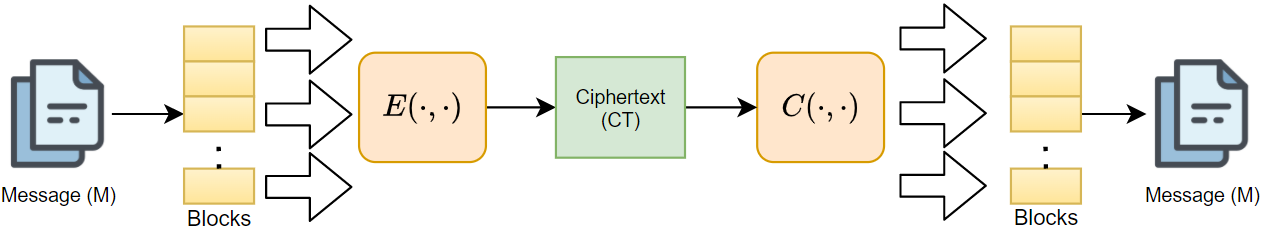
\includegraphics[width=\linewidth]{image/blockcipher.png}
    \caption{Block Cipher Scheme}
    \label{fig:blkcipher}
\end{figure}
\section{Funzionamento di Base}
L'idea alla base dei block cipher è quella di dividere il messaggio in blocchi di dimensione specifica che vengono poi cifrati con una chiave $K$. Inoltre, ogni algoritmo di questo tipo \textbf{deve} implementare una logica di \textbf{pseudo-random permutation}, basata sulla dimensione della chiave usata. Tale permutazione deve avere le seguenti proprietà:
\begin{property}[Pseudo Random Permutation]
\begin{itemize}
    \item \textbf{Biettiva e Reversibile:} dato un input abbiamo un solo output e dato un output dobbiamo poter risalire all'input.
    \item \textbf{Associazione Pseudo-Random:} l'associazione fra i caratteri di partenza con quelli di arrivo deve essere una permutazione casuale. 
\end{itemize}
\end{property}
Il problema di avere una funzione biettiva, è che se un messaggio una volta diviso in blocchi presentasse due blocchi uguali, avremmo uno stesso testo cifrato per quei due blocchi. Stesso discorso se cifriamo due volte lo stesso messaggio.\\
Questo è il funzionamento della modalità \textbf{ECB} \textit{(Electronic Code Book)} , che non va mai usato perché \textbf{perdiamo semantic security}.
\begin{figure}[H]
    \centering
    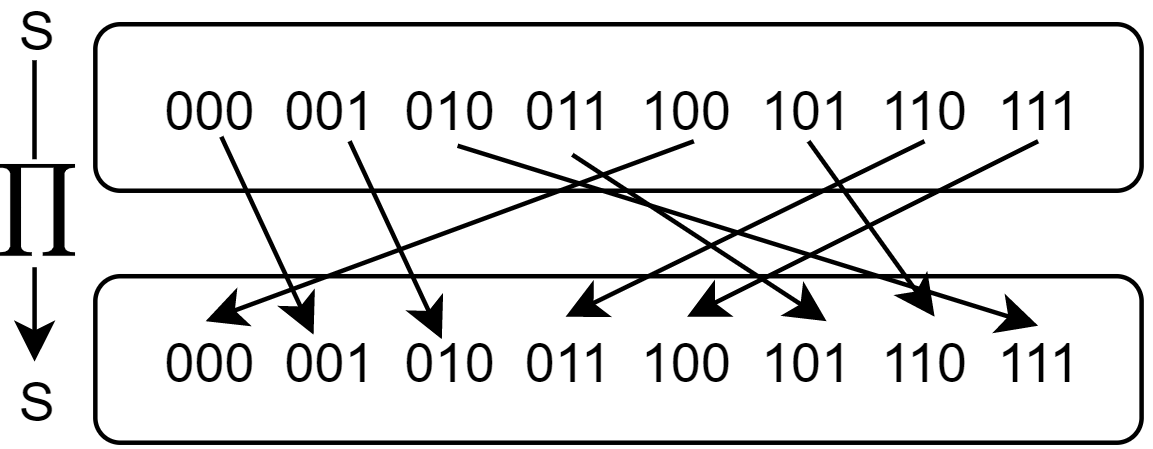
\includegraphics[width=0.8\linewidth]{image/shortcycle.png}
    \caption{PRP function for 3-bit blocks}
    \label{fig:shortcycle}
\end{figure}
\begin{remark}Supponiamo di avere una chiave di dimensione $n=3$bit. L'insieme di tutti i plaintext possibili è di dimensione 8, quindi le permutazioni possibili sono $2^3!=8!=40320$.\\
Se consideriamo \textit{AES} la dimensione della chiave è di 128 bit, quindi il numero di permutazioni è incredibilmente elevato. 
\end{remark}
\begin{remark}In realtà in \textit{AES} le permutazioni sono di meno, perché vengono richieste delle proprietà aggiuntive.
\end{remark}
Una possibile soluzione per ovviare al problema descritto sopra è ovviamente quello di inserire degli \textit{initialization vectors} per nascondere il plaintext al momento dell'applicazione della funzione di \textbf{PRP} \textit{(pseudorandom permutation)} secondo il seguente schema:
\begin{figure}[H]
    \centering
    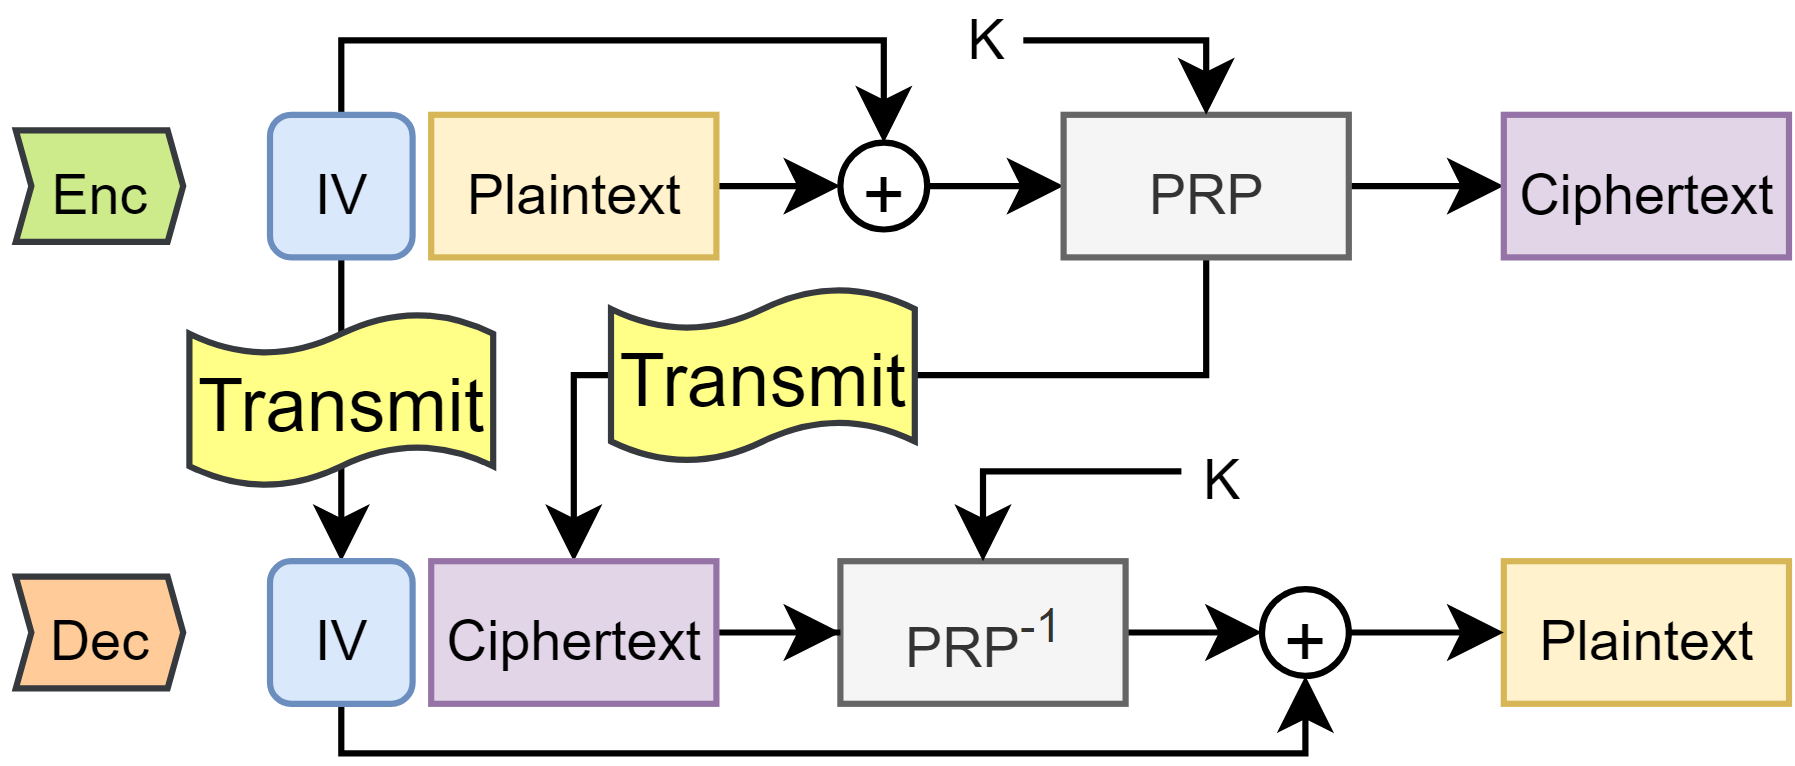
\includegraphics[width=\linewidth]{image/blockiv.png}
    \caption{Block Cipher with IV}
    \label{fig:blockiv}
\end{figure}
Le proprietà che adesso dobbiamo richiedere per gli IV sono due:
\begin{theorem}[Semantic Security for ECB]
Se le seguenti proprietà sono soddisfatte abbiamo sicurezza semantica \textit{ECB}.
\begin{property}[IV properties in Block Ciphers]
\begin{itemize}
    \item Gli IV \textbf{NON} devono \textbf{MAI RIPETERSI}.
    \item Gli IV \textbf{DEVONO} essere \text{NON PREDICIBILI}.
\end{itemize}
\end{property}
A patto che:
\begin{itemize}
    \item Il messaggio è più piccolo di un blocco e non si ripete mai.
    \item Gli IV per messaggi ripetuti hanno valori casuali e sono della stessa dimensione di un blocco.
    \item Per messaggi più lunghi di un blocco bisogna combinare i blocchi per non costruire diversi ciphertext.
\end{itemize}
\begin{remark}
L'inconveniente è che dobbiamo trasmettere un messaggio di dimensione doppia: n bit di ciphertext più n di IV. 
\end{remark}
\end{theorem}
\section{Modes of Operations}
I block ciphers vengono suddivisi in categorie in base alla loro \textit{"Modalità di Operazione"}. Le più usate sono \textbf{CBC} e \textbf{CTR} mentre quelle consigliate da usare sono \textbf{CFB} e \textbf{OFB} per alcune particolari proprietà. Ci sono anche due modalità avanzate che forniscono \textit{authenticated encryption}: \textbf{GCM} e \textbf{OCB}.
\begin{remark}
Ricordiamo che il problema fondamentale è che gli IV non devono mai ripetersi, quindi è necessario ridurne la generazione, oltre che l'overhead sulla trasmissione.
\end{remark}

\subsection{Cipher Block Chaining: CBC}
Questa modalità si basa su un sistema di block-chain descritto nel modo seguente:
\begin{definition}[Encryption with Cipher Block Chaining Mode]\label{def:cbcenc}
\begin{algorithmic}[1]
\State Divide the plaintext in $n$ chunks.
\State $c[0] = PRP(K,IV\oplus m[0])$\Comment{The IV must be truly rnd}
\For{$i=1$ to $n-1$}
    \State $c[i] = PRP(K, c[i-1]\oplus c[i])$\Comment{$c[i-1]$ is used as IV for $c[i]$}
\EndFor
\State Send \textbf{IV} along with the \textbf{ciphertexts}.
\end{algorithmic}
\end{definition}
Se l\textbf{'IV} è \textbf{truly random} il meccanismo \textbf{è semantic secure} in quanto il primo ciphertext generato sarà una quantità che può essere vista come casuale e tale randomicità verrà trasportata anche ai ciphertext successivi. Pertanto, \textbf{con un solo IV inviato possiamo garantire sicurezza semantica per tutto il messaggio}.\\
Tuttavia le \textbf{cifrature} \textbf{non} sono \textbf{parallelizabili} in quanto le cifrature \textit{i-esime} dipendono da quella successiva e l'ordine delle cifrature è quindi fondamentale. 
\begin{definition}[Decryption with Cipher Block Chaining Mode]\label{def:cbcdec}
\begin{algorithmic}[1]
\State $m[0]=IV\oplus PRP(K,c[0])$
\For{$i=1$ to $n-1$}
\State $m[i] = c[i-1]\oplus PRP(K, c[i])$
\EndFor
\end{algorithmic}
\end{definition}
Osserviamo che il discorso sulla parallelizzazione non sussiste per la decrittazione, in quanto con il solo IV e il messaggio è possibile decifrare tutto il ciphertext in parallelo.
\begin{figure}[ht]
    \centering
    \begin{subfigure}[b]{0.48\textwidth}
    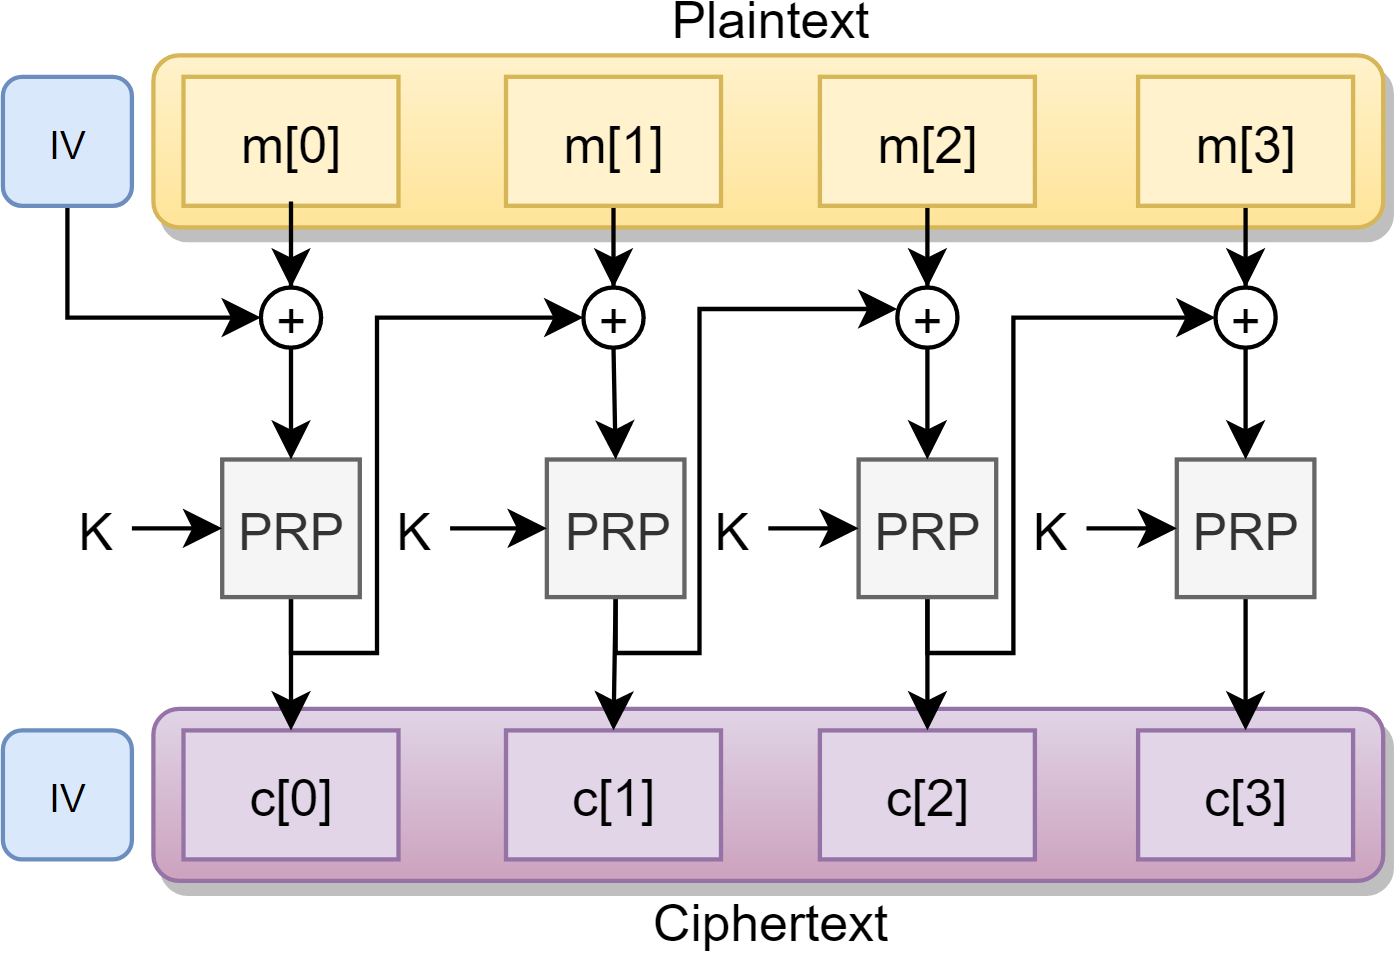
\includegraphics[width=\textwidth]{image/cbcenc.png}
    \caption{CBC Encryption}
    \label{fig:cbcenc}
    \end{subfigure}\quad
    \begin{subfigure}[b]{0.48\textwidth}
    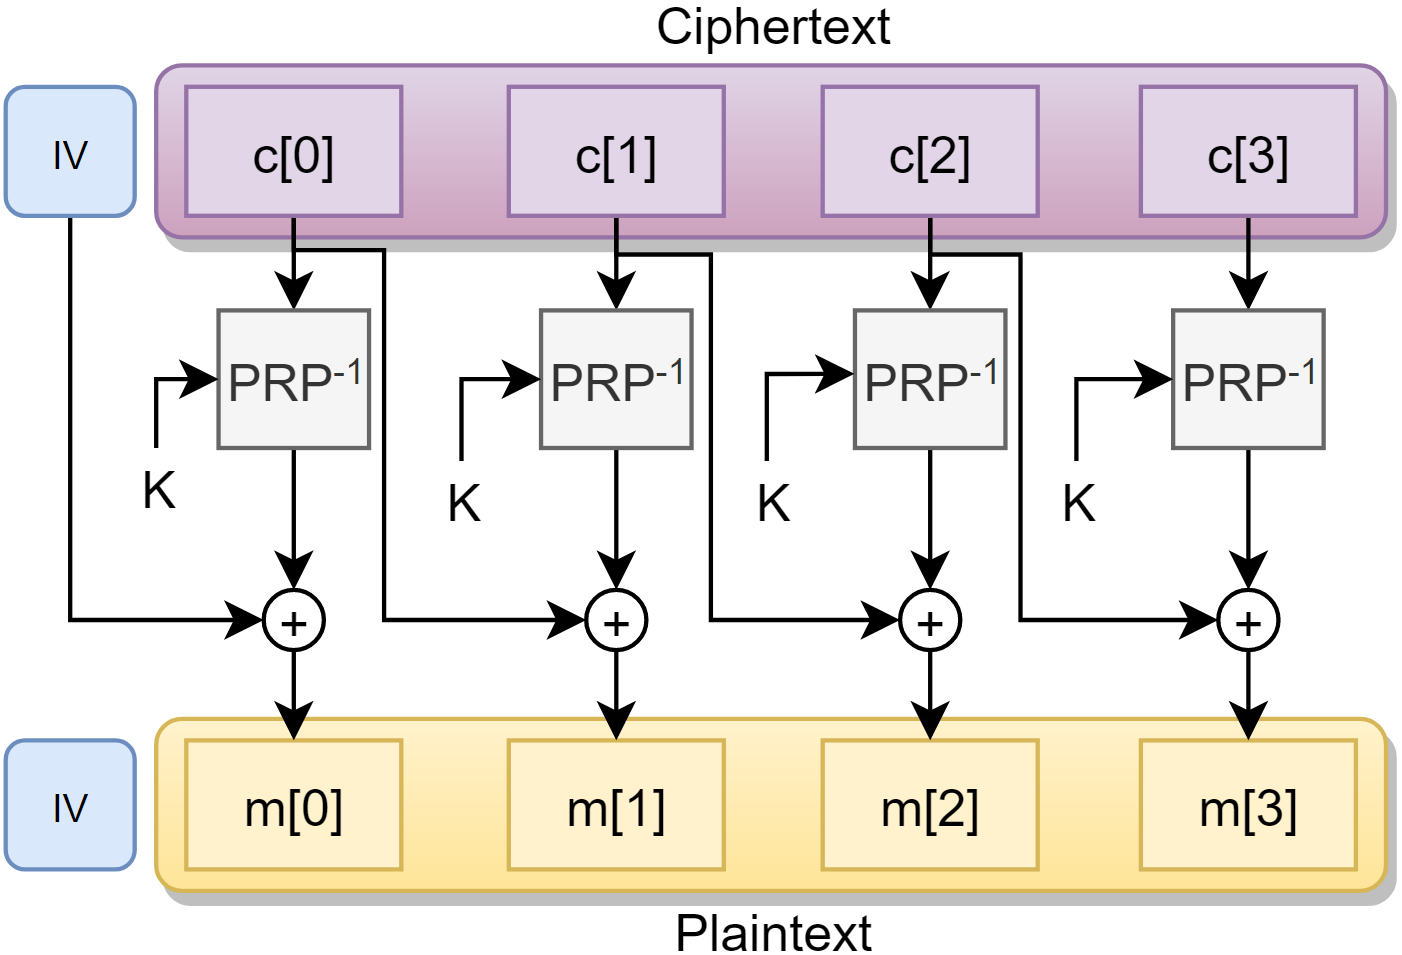
\includegraphics[width=\textwidth]{image/cbcdec.png}
    \caption{CBC Decryption}
    \label{fig:cbcdec}
    \end{subfigure}
    \caption{CBC Mode}
\end{figure}
\begin{remark}
CBC è il sistema più comune e usato per cifrare dei messaggi, ma è sicuro sempre se e solo se la nonce è \textbf{truly random e non predicibile}.
\end{remark}
\begin{remark}
IV predicibili possono portare a CPA, come successo in \textbf{BEAST} nel 2011.
\end{remark}
\begin{remark}
L'implementazione di CBC richiede due circuiti differenti per cifrare e decifrare i messaggi. Poiché questi meccanismi sono spesso inseriti a livello hardware, usare due circuiti significa usare il doppio dello spazio per la realizzazione del sistema di cifratura.
\end{remark}
\begin{remark}
Poiché lo xor impone che le dimensioni dei chunk siano di un numero fissato, è necessario fare un padding per messaggi che non sono multipli del numero di byte scelto. Il padding viene calcolato secondo degli standard, un esempio è \textbf{PKCS\#7}.
\end{remark}
\subsection{Cipher Feedback Mode e Output Feedback Mode}
Le modalità CFB e OFB offrono un punto di vista differente rispetto a CBC. In particolare, tendono ad imitare gli stream ciphers, producendo un keystream utile alla cifratura del plaintext, permettendo di usare un solo circuito, sia per \textit{PRP} che per \textit{PRP\textsuperscript{-1}}.
\begin{definition}[Cipher Feedback Mode - CFB [Encryption]]\label{alg:cfb}
\begin{algorithmic}[1]
\State Assume we have $n$ plaintexts $m[i]\,i=1,\dots,n$.
\State $K_s=\text{ENC}(key, IV)$\Comment{The IV must be truly rnd}
\State $c[0]=m[0]\oplus{K_s}$\Comment{encrypt as stream ciphers with keaystream}
\For{$i=1$ to $n-1$}
    \State $K_s=\text{ENC}(key, c[0])$
    \State $c[i] = c[i-1]\oplus K_s$\Comment{$c[i-1]$ is used as IV for $c[i]$}
\EndFor
\State Send \textbf{IV} along with the \textbf{ciphertexts}.
\end{algorithmic}
\end{definition}
\begin{definition}[Output Feedback Mode - OFB [Encryption]]\label{alg:ofb}
\begin{algorithmic}[1]
\State Assume we have $n$ plaintexts $m[i]\,i=1,\dots,n$.
\State $K_s[0]=\text{ENC}(key, IV)$\Comment{The IV must be truly rnd}
\For{$i=0$ to $n$}
    \State $c[i]=m[0]\oplus{K_s}$\Comment{encrypt as stream ciphers with keaystream}
    \State $K_s[i]=\text{ENC}(key, K_s[i-1])$ \Comment{$K_s[i-1]$ is used as IV for $K_s[i]$}
\EndFor
\State Send \textbf{IV} along with the \textbf{ciphertexts}.
\end{algorithmic}
\end{definition}
Sia CFB che OFB cifrano il messaggio mascherandolo con un keystream generato tramite un \textbf{\textit{block cipher encryptiion}} senza la necessità di fare padding. L'\textbf{encryption non} è \textbf{parallelizzabile} in nessuno dei due casi ma \textbf{OFB permette} di fare \textbf{preprocessing} in quanto lo stato del messaggio cifrato non dipende da quello precedente e i keystream possono essere calcolati in blocco.\\
Per fare decryption è possibile usare lo stesso circuito di encryption, dove \textbf{CFB} è in vantaggio perché \textbf{permette} di \textbf{parallelizzare} il processo.
\begin{definition}[CFB Decryption]
\begin{algorithmic}[1]
\State Assume we have \textit{n} ciphertexts.
\State Take the \textit{IV} from arriving message.
\State $K_s[0] = ENC(IV, k)$
\ForAll{ciphertexts}
\State $m[i] = K_s[i-1]\oplus{c[i]}$\Comment{Get the Plaintext}
\State $K_s[i] = ENC(c[i-1], k)$\Comment{Generate Keystream from $c[i-1]$}
\EndFor
\end{algorithmic}
\end{definition}
\begin{definition}[OFB Decrption]
\begin{algorithmic}[1]
\State Assume we have \textit{n} ciphertexts.
\State Take \textit{IV} from arriving message.
\State $K_s[0] = ENC(IV, k)$
\ForAll{ciphertexts}
\State $m[i] = K_s[i-1]\oplus{c[i]}$\Comment{Get the Plaintext}
\State $K_s = ENC(K_s[i-1], K)$\Comment{Generate Keystream from $K_s[i-1]$}
\EndFor
\end{algorithmic}
\end{definition}
\begin{figure}[h]
    \centering
    \begin{subfigure}[b]{0.48\textwidth}
    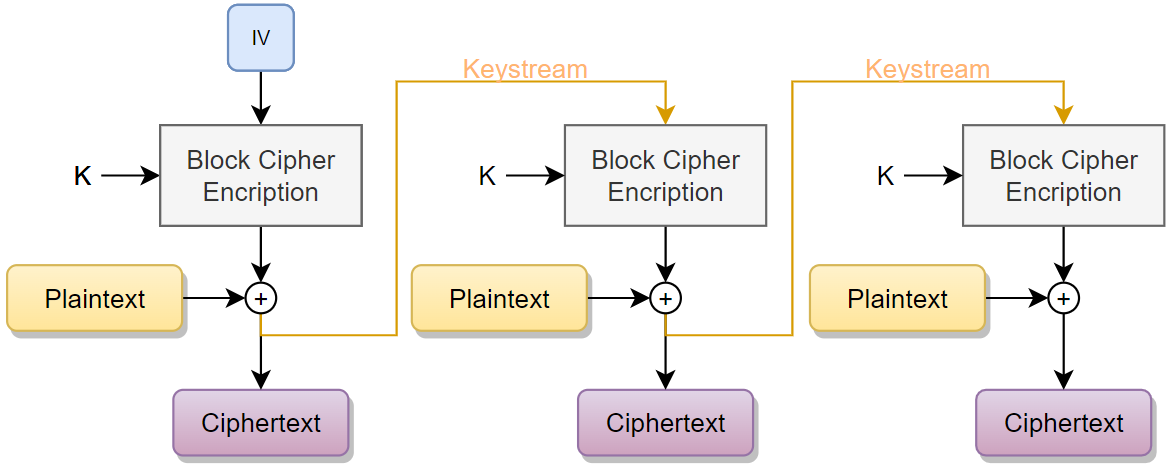
\includegraphics[width=\textwidth]{image/cfbenc.png}
    \caption{Encryption}
    \label{fig:cfbenc}
    \end{subfigure}\quad
    \begin{subfigure}[b]{0.48\textwidth}
    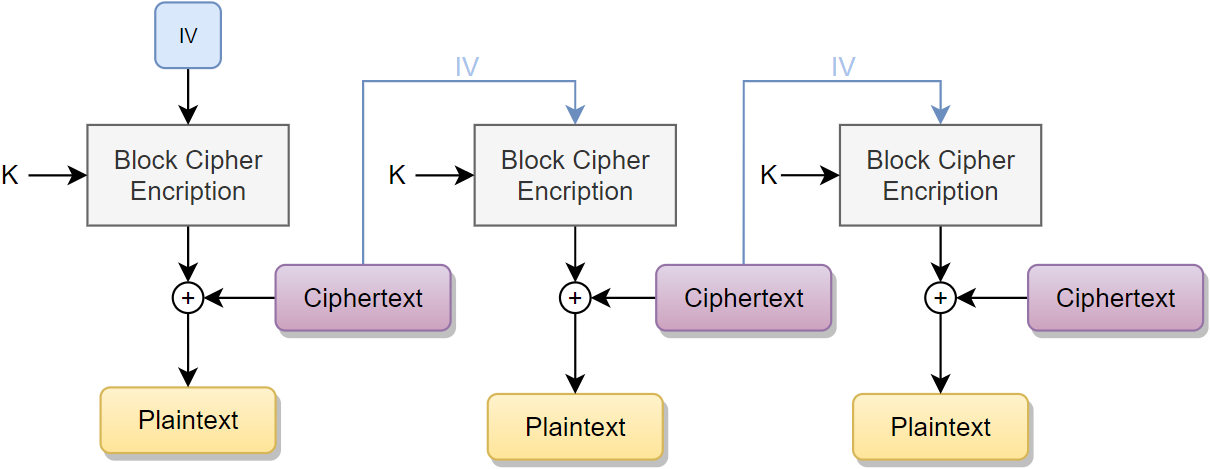
\includegraphics[width=\textwidth]{image/cfbdec.png}
    \caption{Decryption}
    \label{fig:cfbdec}
    \end{subfigure}
    \caption{Cipher Feedback Mode}
\end{figure}
\begin{figure}[H]
    \centering
    \begin{subfigure}[b]{0.48\textwidth}
    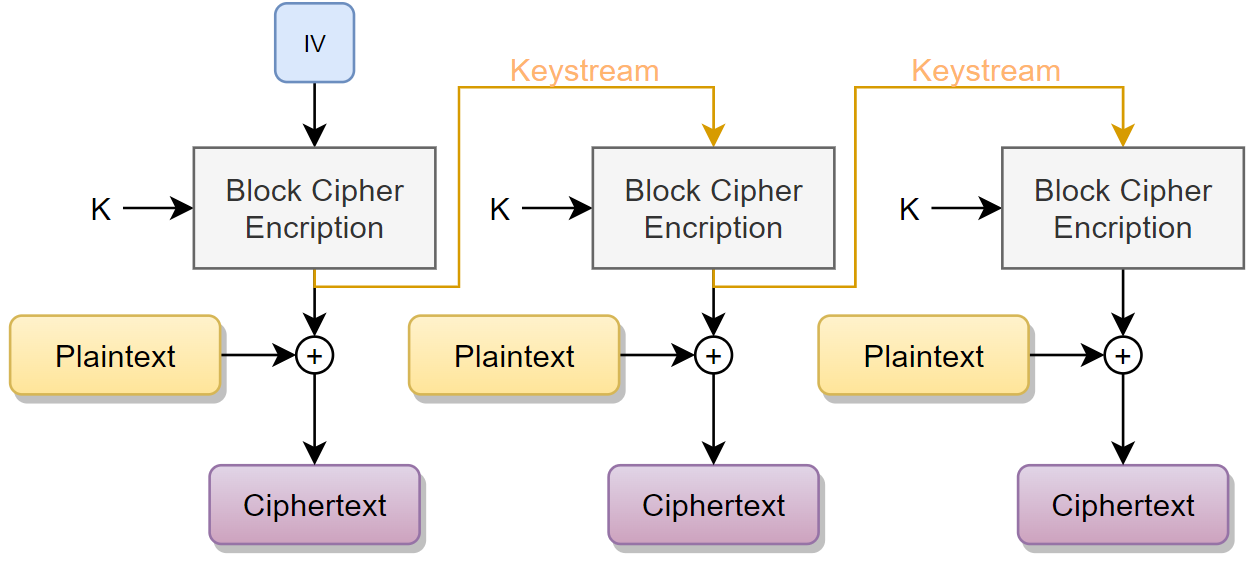
\includegraphics[width=\textwidth]{image/ofbenc.png}
    \caption{Encryption}
    \label{fig:ofbenc}
    \end{subfigure}\quad
    \begin{subfigure}[b]{0.48\textwidth}
    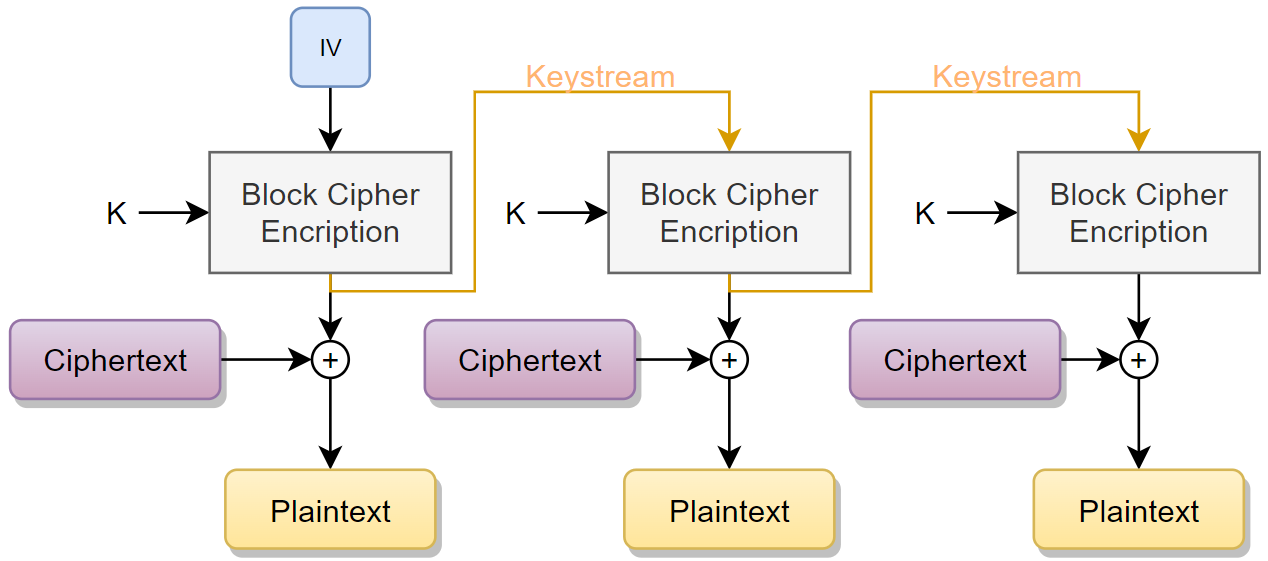
\includegraphics[width=\textwidth]{image/ofbdec.png}
    \caption{Decryption}
    \label{fig:ofbdec}
    \end{subfigure}
    \caption{Output Feedback Mode}
\end{figure}
\section{Short Cycle Problem}
I cifratori a blocchi dipendono fortemente dal blocco di encryption che calcola la pseudorandom permutation. Questo implica che la funzione che scegliamo per calcolare la permutazione deve essere fatta bene e robusta anche a specifiche condizioni iniziali. In particolare, non possiamo usare funzioni che soffrono del:
\begin{definition}[Short Cycle Problem]\label{def:shortcycle}
Condizione per la quale un algoritmo di cifratura, a partire da alcune specifiche condizioni iniziali, tendono a ripetere i valori di ciphertext dopo poco tempo.
\end{definition}
\begin{example} Consideriamo l'insieme $S$ e la permutazione seguente $\prod$.
\begin{enumerate}
    \item \textbf{OFB} con $IV=010$: $C=010\,111\,100\,001$ \textcolor{red}{$010\,111\,\dots$}\\
    I valori di $C$ cominciano a ripetersi dopo 5 iterazioni.
    \item \textbf{OFB} con $IV=011$: $C=011\,101\,110$ \textcolor{red}{$011\,101\,110\,\dots$}\\
    I valori di $C$ cominciano a ripetersi dono 3 iterazioni.
\end{enumerate}
\end{example}
\begin{example}Vediamo che anche \textbf{CBC} presenta gli stessi problemi se cifra un testo con delle ripetizioni: 
\begin{itemize}
    \item $P=011\,011\,011$ con $IV:010$: \textcolor{red}{$C=(010)\,010\,010\,010$}
\end{itemize}
\end{example}
\section{Counter Mode}
Poiché le modalità precedenti sono soggette allo \textit{short cycle problem} una modalità resistente è necessaria. In particolare, poiché il problema è intrinseco all'\textit{IV} scelto per avviare la cifratura, se questo fosse sviluppato dinamicamente e sempre diverso, non potremmo avere cicli all'interno di una sequenza di cifratura.\\
Assumendo l'\textit{IV} come un \textbf{contatore} incrementato ad ogni nuovo blocco, è possibile dimostrare che se la PRP è sicura, allora il risultato pseudorandomico generato è sicuro.
\begin{remark}
La modalità \textit{CTR} gode della maggior parte dei vantaggi:
\end{remark}
\begin{enumerate}
    \item [\textcolor{green}{\checkmark}]Trasforma i block-cipher in stream-cipher.
    \item [\textcolor{green}{\checkmark}]Combina i vantaggi di \textit{CFB}(\cref{alg:cfb}) e \textit{OFB}(\cref{alg:ofb}).
    \item [\textcolor{green}{\checkmark}]Permette un'implementazione efficiente (sia \textit{HW} che \textit{SW}) utilizzando parallelizzazione sia in encryption che decryption.
    \item [\textcolor{green}{\checkmark}]Richiede l'implementazione di un singolo blocco di cifratura per entrambe le operazioni.
    \item [\textcolor{green}{\checkmark}]Permette di attuare meccanismi di \textbf{Random Access} (ad esempio a sistemi di memoria cifrata) poiché la decrittazione del blocco \textit{i-esimo} non dipende dai precedenti.
    \item [\textcolor{green}{\checkmark}]E' sicuro se usiamo accortezze sui contatori.
    \item [\textcolor{green}{\checkmark}]Viene garantita robustezza allo Short Cycle Problem (\cref{def:shortcycle}).
\end{enumerate}
\begin{definition}[Counter Mode Encryption/Decription]\label{def:ctrmode}
\begin{algorithmic}[1]
\State Assume we have \textit{n} plaintext/ciphertext
\State Initialize a counter $ctr$ as standard specifies\footnotemark.
\ForAll{plaintexts}
\State $K_s[i] = ENC(ctr,K)$
\State $c[i] = K_s[i]\oplus{m[i]}$
\State $ctr = ctr + 1$
\EndFor
\end{algorithmic}
\footnotetext{\textsuperscript{\thefootnote}Ad esempio AES-CTR specifica che per l'\textbf{Initial Counter Block} il contatore è formato \textbf{da 128bit} dove i \textbf{primi 96} sono costituiti dall'\textbf{IV} e i \textbf{restanti 32} dal \textbf{contatore}, \textbf{partendo da 1}.}
\end{definition}
\begin{figure}[H]
    \centering
    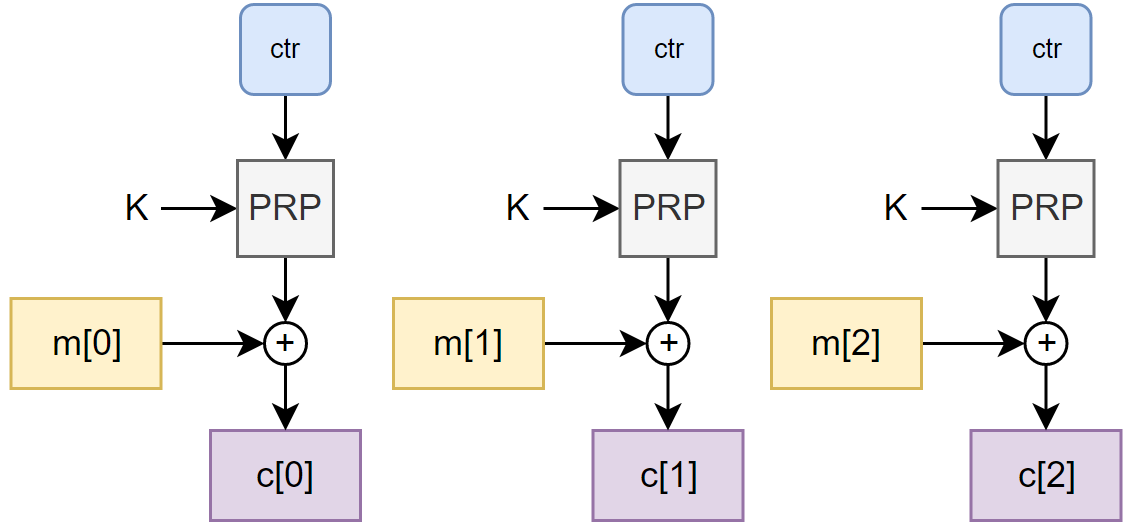
\includegraphics[width=\linewidth]{image/blkctr.png}
    \caption{Counter Mode Block Cipher}
    \label{fig:ctrmode}
\end{figure}

